\documentclass{article}

%% Created with wxMaxima 12.01.0

\setlength{\parskip}{\medskipamount}
\setlength{\parindent}{0pt}
\usepackage[utf8]{inputenc}
\usepackage{graphicx}
\usepackage{color}
\usepackage{amsmath}

\definecolor{labelcolor}{RGB}{100,0,0}

\begin{document}

\noindent
%%%%%%%%%%%%%%%
%%% INPUT:
\begin{minipage}[t]{8ex}{\color{red}\bf
\begin{verbatim}
(%i23) 
\end{verbatim}}
\end{minipage}
\begin{minipage}[t]{\textwidth}{\color{blue}
\begin{verbatim}
E:180;
Vm:230*sqrt(2),numer;
a:45*%pi/180;
R:12;
L:22*10^-3;
w:50*2*%pi,numer;
b:atan(w*L/R),numer;
z:sqrt(R^2+(w*L)^2),numer;
V(wt):=Vm*sin(wt+a);
C:(E/R)-Vm/z*sin(a-b),numer;
ti:-0.1;
tf:2*%pi;
\end{verbatim}}
\end{minipage}
%%% OUTPUT:
\begin{math}\displaystyle
\parbox{8ex}{\color{labelcolor}(\%o23) }
180
\end{math}

\begin{math}\displaystyle
\parbox{8ex}{\color{labelcolor}(\%o24) }
325.2691193458119
\end{math}

\begin{math}\displaystyle
\parbox{8ex}{\color{labelcolor}(\%o25) }
\frac{\pi }{4}
\end{math}

\begin{math}\displaystyle
\parbox{8ex}{\color{labelcolor}(\%o26) }
12
\end{math}

\begin{math}\displaystyle
\parbox{8ex}{\color{labelcolor}(\%o27) }
\frac{11}{500}
\end{math}

\begin{math}\displaystyle
\parbox{8ex}{\color{labelcolor}(\%o28) }
314.1592653589793
\end{math}

\begin{math}\displaystyle
\parbox{8ex}{\color{labelcolor}(\%o29) }
0.5225544346474
\end{math}

\begin{math}\displaystyle
\parbox{8ex}{\color{labelcolor}(\%o30) }
13.84806431604333
\end{math}

\begin{math}\displaystyle
\parbox{8ex}{\color{labelcolor}(\%o31) }
\mathrm{V}\left( wt\right) :=Vm\,\mathrm{sin}\left( wt+a\right) 
\end{math}

\begin{math}\displaystyle
\parbox{8ex}{\color{labelcolor}(\%o32) }
8.89705939289934
\end{math}

\begin{math}\displaystyle
\parbox{8ex}{\color{labelcolor}(\%o33) }
-0.1
\end{math}

\begin{math}\displaystyle
\parbox{8ex}{\color{labelcolor}(\%o34) }
2\,\pi 
\end{math}
%%%%%%%%%%%%%%%


\noindent
%%%%%%%%%%%%%%%
%%% INPUT:
\begin{minipage}[t]{8ex}{\color{red}\bf
\begin{verbatim}
(%i39) 
\end{verbatim}}
\end{minipage}
\begin{minipage}[t]{\textwidth}{\color{blue}
\begin{verbatim}
i(wt):=C*%e^(-R/(L*w)*wt)+Vm/z*sin(wt+a-b)-(E/R);
Vt(wt):=if i(wt)>0 then V(wt) else 0;
wxplot2d([i(wt)],[wt,ti,tf],[y,-40,10],[gnuplot_preamble, "set grid"]);
\end{verbatim}}
\end{minipage}
%%% OUTPUT:
\begin{math}\displaystyle
\parbox{8ex}{\color{labelcolor}(\%o39) }
\mathrm{i}\left( wt\right) :=C\,{e}^{\frac{-R}{L\,w}\,wt}+\frac{Vm}{z}\,\mathrm{sin}\left( wt+a-b\right) -\frac{E}{R}
\end{math}

\begin{math}\displaystyle
\parbox{8ex}{\color{labelcolor}(\%o40) }
\mathrm{Vt}\left( wt\right) :=\mathrm{if} \mathrm{i}\left( wt\right) >0 \mathrm{then} \mathrm{V}\left( wt\right)  \mathrm{else} 0
\end{math}

\begin{math}\displaystyle
\parbox{8ex}{\color{labelcolor}(\%t41) }
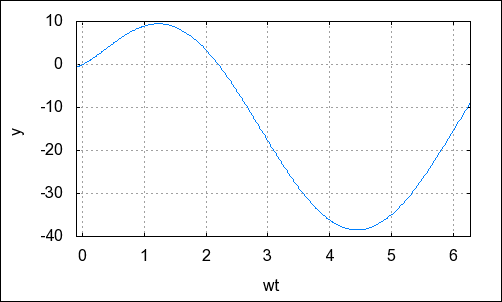
\includegraphics[width=9cm]{problema_2_9_img/problema_2_9_1.png}
\end{math}

\begin{math}\displaystyle
\parbox{8ex}{\color{labelcolor}(\%o41) }

\end{math}
%%%%%%%%%%%%%%%


\noindent
%%%%%%%%%%%%%%%
%%% INPUT:
\begin{minipage}[t]{8ex}{\color{red}\bf
\begin{verbatim}
(%i42) 
\end{verbatim}}
\end{minipage}
\begin{minipage}[t]{\textwidth}{\color{blue}
\begin{verbatim}
wxplot2d([V(wt), Vt(wt)],[wt,ti,tf],[y,-350,350],[gnuplot_preamble, "set grid"]);
\end{verbatim}}
\end{minipage}
%%% OUTPUT:
\begin{math}\displaystyle
\parbox{8ex}{\color{labelcolor}(\%t42) }
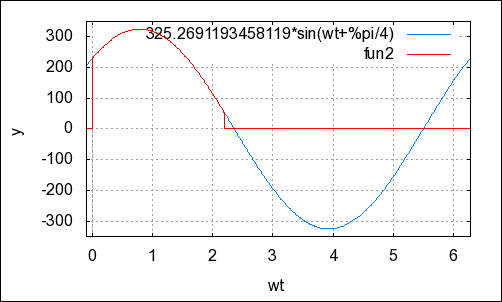
\includegraphics[width=9cm]{problema_2_9_img/problema_2_9_2.png}
\end{math}

\begin{math}\displaystyle
\parbox{8ex}{\color{labelcolor}(\%o42) }

\end{math}
%%%%%%%%%%%%%%%

\end{document}
